\begin{frame}
	\frametitle{Sinais Digitais e Sub-amostragem (Downsampling)}
	\begin{figure}
		\centering
		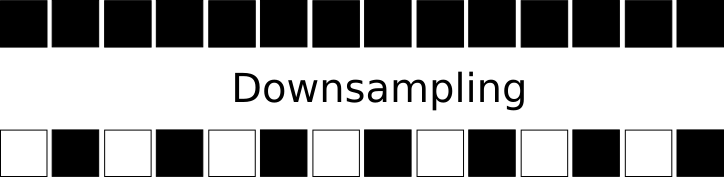
\includegraphics[width=0.5\linewidth]{../monography/images/downsampling}
		\caption{Sub-amostragem}
		\label{fig:downsampling}
	\end{figure}
	\par Mesmo depois de amostrados e quantizados \cite{haykin2011sistemas} os sinais de EEG e voz, na maioria das vezes, precisam ser sub-amostrados para que se sejam viáveis o processamento e o armazenamento\cite{robi2003}.
	
	\par Além disso o \textit{downsampling} será fundamental no uso das transformadas \textit{wavelet}.
\end{frame}